\documentclass[a4paper, 12pt]{article}
%\documentclass[a4paper, 14pt]{extarticle}
\usepackage[utf8]{inputenc}
\usepackage[english,russian]{babel}
\usepackage{indentfirst}

\usepackage[utf8]{inputenc}%включаем свою кодировку: koi8-r или utf8 в UNIX, cp1251 в Windows
\usepackage[english,russian]{babel}%используем русский и английский языки с переносами
\usepackage{amssymb,amsfonts,amsmath,mathtext,enumerate,float} %подключаем нужные пакеты расширений
\usepackage{graphicx}
\usepackage{cmap}
\usepackage{verbatim}
\usepackage{wrapfig}
%\usepackage[T2A]{fontenc}
\graphicspath{{imgs/}}%путь к рисункам
%\usepackage{enumitem}
%\setlist{nolistsep}

\usepackage{geometry} % Меняем поля страницы
\geometry{left=3cm}% левое поле
\geometry{right=2cm}% правое поле
\geometry{top=2cm}% верхнее поле
\geometry{bottom=2cm}% нижнее поле

\geometry{marginparwidth=2.5cm} % Ширина заметок на полях.

\usepackage{cite}

\makeatletter
\renewcommand{\@biblabel}[1]{#1.} % Заменяем библиографию с квадратных скобок на точку:
\makeatother

\usepackage{float}
\usepackage{xcolor}
\usepackage{marginnote}
\reversemarginpar % Перенос заметок с правого поля на левое.

\usepackage{tabularx}

% Полезные типы колонок: колонки с выравниваем влево/по центру/справа 
% фиксированной ширины (как p{}, но не justify).
\newcolumntype{L}[1]{>{\raggedright\let\newline\\\arraybackslash\hspace{0pt}}m{#1}}
\newcolumntype{C}[1]{>{\centering\let\newline\\\arraybackslash\hspace{0pt}}m{#1}}
\newcolumntype{R}[1]{>{\raggedleft\let\newline\\\arraybackslash\hspace{0pt}}m{#1}}

% Колонки для tabularx
\newcolumntype{E}[1]{>{\hsize=#1\hsize\raggedright\arraybackslash}X}%
\newcolumntype{F}[1]{>{\hsize=#1\hsize\centering\arraybackslash}X}%
\newcolumntype{G}[1]{>{\hsize=#1\hsize\raggedleft\arraybackslash}X}%
%\newcolumntype{C}[2]{>{\hsize=#1\hsize\columncolor{#2}\centering\arraybackslash}X}%

\usepackage{indentfirst}
\usepackage{setspace}
\onehalfspacing

% % % % % % % % % % % % % % % % % % %
% Нумерация абзацев
% % % % % % % % % % % % % % % % % % %

\renewcommand{\theenumi}{\arabic{enumi}}% Меняем везде перечисления на цифра.цифра
%\renewcommand{\labelenumi}{\arabic{enumi}}% Меняем везде перечисления на цифра.цифра
\renewcommand{\theenumii}{.\arabic{enumii}}% Меняем везде перечисления на цифра.цифра
\renewcommand{\labelenumii}{\arabic{enumi}.\arabic{enumii}.}% Меняем везде перечисления на цифра.цифра
\renewcommand{\theenumiii}{.\arabic{enumiii}}% Меняем везде перечисления на цифра.цифра
\renewcommand{\labelenumiii}{\arabic{enumi}.\arabic{enumii}.\arabic{enumiii}.}% Меняем везде перечисления на цифра.цифра

\renewcommand{\thesection}{\arabic{section}}
%\renewcommand{\thesubsection}{\arabic{subsection}}
%\renewcommand{\thesubsubsection}{\arabic{subsubsection}}
\setlength{\intextsep}{1.75\intextsep}
\setcounter{secnumdepth}{5}
\setcounter{tocdepth}{5}
%\addtolength{\parskip}{8pt}


% % % % % % % % % % % % % % % % % % %
% Новые команды
% % % % % % % % % % % % % % % % % % %

\newcommand{\off}[1]{{\color{gray}#1}}

%\newcommand{\todo}[1]{\marginpar{\color{red} \footnotesize #1}}
%\newcommand{\todonote}[1]{\todo{#1}}
%\newcommand{\toask}[1]{\marginpar{\color{blue} \footnotesize #1}}

%\newcommand{\todo}[1]{}
%\newcommand{\todonote}[1]{{\color{red}#1}}
%\newcommand{\toask}[1]{{\color{blue}#1}}

\newcommand{\todo}[1]{}
\newcommand{\todonote}[1]{}
\newcommand{\toask}[1]{}


\newcommand{\comm}[1]{\marginpar{\color{red}\Large \textbf{!!}}}
\newcommand{\alt}[2]{$\overset{\text{#2}}{\text{#1}}$}
\newcommand{\tweakedsim}{{\raise.17ex\hbox{$\scriptstyle\sim$}}}
\newcommand{\ceil}[1]{\left\lceil#1\right\rceil}
\newcommand{\abs}[1]{\left|#1\right|}
\renewcommand{\phi}{\varphi}

% % % % % % % % % % % % % % % % % % %
% Библиография
% % % % % % % % % % % % % % % % % % %

%\usepackage[backend=biber,style=unsrt]{biblatex}
%\addbibresource{bibliography.bib}

%\bibliographystyle{unsrt}

% https://tex.stackexchange.com/questions/26575/bibtex-how-can-i-automatically-reduce-long-author-lists-to-xxx-et-al
%\bibliographystyle{unsrtLimauthors.bst}
\bibliographystyle{ugost2008}


\let\stdsection\section
\renewcommand\section{\newpage\stdsection}

\begin{document}
%\maketitle
\newcommand{\fnt}[1]{\fontsize{#1}{\baselineskip}\selectfont}
% Ставим одинарный междустрочный интервал
\singlespacing
% Ставим геометрию для титульной страницы.
\newgeometry{left=3cm,right=1.5cm,top=2cm,bottom=2cm}

% Просто информация. Нигде в странице не используется, но зато попадёт в pdf info.
\author{Мингулов К.\:Т.}
\title{Пакет DREAM: автоматизация метода многопетлевых вычислений, основанного на рекуррентных соотношениях по размерности пространства-времени}
\date{2020 г.}

\begin{titlepage}

%%%%%%%%%%%%%%%%%%%%%%%%%%%%%%%%%%%%%%%%%%%%%%%%%%%%%%%%%%%%%%%%%%%%%%%%%%%%%%%%

\begin{center}
    {\fnt{10.5} МИНИСТЕРСТВО ОБРАЗОВАНИЯ И НАУКИ РОССИЙСКОЙ ФЕДЕРАЦИИ} \\
        \vspace{0.3\baselineskip}
    {\fnt{10.5} ФЕДЕРАЛЬНОЕ ГОСУДАРСТВЕННОЕ АВТОНОМНОЕ ОБРАЗОВАТЕЛЬНОЕ \\ 
		\vspace{-0.3\baselineskip}
		УЧРЕЖДЕНИЕ ВЫСШЕГО ОБРАЗОВАНИЯ} \\
        \vspace{0.3\baselineskip}
    {\fnt{10.5} <<НОВОСИБИРСКИЙ НАЦИОНАЛЬНЫЙ ИССЛЕДОВАТЕЛЬСКИЙ ГОСУДАРСТВЕННЫЙ \\
		\vspace{-0.3\baselineskip}
		УНИВЕРСИТЕТ>> (НОВОСИБИРСКИЙ ГОСУДАРСТВЕННЫЙ УНИВЕРСИТЕТ, НГУ)}
\end{center}

%%%%%%%%%%%%%%%%%%%%%%%%%%%%%%%%%%%%%%%%%%%%%%%%%%%%%%%%%%%%%%%%%%%%%%%%%%%%%%%%

\vspace{0.5\baselineskip}

\noindent
{\fnt{11}Факультет}
$\overset{\text{\fnt{11}\textbf{ФИЗИЧЕСКИЙ}}\phantom{\hspace{10.9cm}}}{\underline{\hspace{0.88\textwidth}}}$

\vspace{0.3\baselineskip}

\noindent
{\fnt{11}Кафедра}
$\overset{\text{\fnt{11}\textbf{ФИЗИКО-ТЕХНИЧЕСКОЙ ИНФОРМАТИКИ}}\phantom{\hspace{4.8cm}}}{\underline{\hspace{0.895\textwidth}}}$

\vspace{1\baselineskip}

\noindent
{\fnt{11}Направление подготовки}
$\overset{\text{\fnt{11}\textbf{03.04.02 ФИЗИКА}}\phantom{\hspace{8cm}}}{\underline{\hspace{0.73\textwidth}}}$

\vspace{0.3\baselineskip}

\noindent
{\fnt{11}Образовательная программа}
$\overset{\text{\fnt{11}\textbf{БАКАЛАВРИАТ}}\phantom{\hspace{7.3cm}}}{\underline{\hspace{0.689\textwidth}}}$

%%%%%%%%%%%%%%%%%%%%%%%%%%%%%%%%%%%%%%%%%%%%%%%%%%%%%%%%%%%%%%%%%%%%%%%%%%%%%%%%

\vspace{\baselineskip}

\begin{center}\bfseries
    {\fnt{11} ВЫПУСКНАЯ КВАЛИФИКАЦИОННАЯ РАБОТА БАКАЛАВРА} \\
        \vspace{0\baselineskip}
    %{\fnt{11} МАГИСТЕРСКАЯ ДИССЕРТАЦИЯ}
\end{center}

%%%%%%%%%%%%%%%%%%%%%%%%%%%%%%%%%%%%%%%%%%%%%%%%%%%%%%%%%%%%%%%%%%%%%%%%%%%%%%%%

\vspace{0.3\baselineskip}

\noindent
$\overset{\text{\fnt{11}Каня Кирилл Олегович}}
{\underset{\text{\fnt{9}(фамилия, имя, отчество автора)}}{\underline{\hspace{\textwidth}}}}$

%%%%%%%%%%%%%%%%%%%%%%%%%%%%%%%%%%%%%%%%%%%%%%%%%%%%%%%%%%%%%%%%%%%%%%%%%%%%%%%%

\vspace{\baselineskip}

\noindent
{\fnt{11}Тема работы}
$\overset{\text{\fnt{11}Разработка ПО для онлайн монитора светимости}}{\underline{\hspace{0.855\textwidth}}}$

\noindent
$\overset{\text{\fnt{11}\hspace{0.16\textwidth}детектора Belle II}}{\underline{\hspace{\textwidth}}}$

\noindent
$\overset{\text{\fnt{11}}}{\underline{\hspace{\textwidth}}}$

%%%%%%%%%%%%%%%%%%%%%%%%%%%%%%%%%%%%%%%%%%%%%%%%%%%%%%%%%%%%%%%%%%%%%%%%%%%%%%%%

\vspace{2\baselineskip}

\noindent
\begin{tabular}{@{}p{0.5\textwidth}@{}@{}R{0.5\textwidth}@{}}
\fnt{11}\textbf{<<К защите допущена>>} &  \\
\fnt{11}Заведующий кафедрой,           & \fnt{11}\textbf{Научный руководитель} \\
\fnt{11}канд. физ.-мат. наук, доцент,   & \fnt{11}канд. физ.-мат. наук, \\
\fnt{11}зав. лаб. ИЯФ СО РАН            & \fnt{11}с.н.с. ИЯФ СО РАН \\
$\overset{\text{\fnt{11}Кроковный, П.\,П.}}{\underset{\text{\fnt{8}(фамилия, И.\,О.)}}{\underline{\hspace{0.225\textwidth}}}}
\overset{\text{\fnt{11}/}}{}
\overset{\text{\fnt{11}}}{\underset{\text{\fnt{8}(подпись)}}{\underline{\hspace{0.125\textwidth}}}}$ &
$\overset{\text{\fnt{11}Ремнев М.\,А.}}{\underset{\text{\fnt{8}(фамилия, И.\,О.)}}{\underline{\hspace{0.225\textwidth}}}}
\overset{\text{\fnt{11}/}}{}
\overset{\text{\fnt{11}}}{\underset{\text{\fnt{8}(подпись)}}{\underline{\hspace{0.125\textwidth}}}}$ \\
$\overset{\text{\fnt{11}<<}}{}
\overset{\text{\fnt{11}}}{\underline{\hspace{0.05\textwidth}}}
\overset{\text{\fnt{11}>>}}{}
\overset{\text{\fnt{11}}}{\underline{\hspace{0.215\textwidth}}}
\overset{\text{\fnt{11}2020 г.}}{}$ & 
$\overset{\text{\fnt{11}<<}}{}
\overset{\text{\fnt{11}}}{\underline{\hspace{0.05\textwidth}}}
\overset{\text{\fnt{11}>>}}{}
\overset{\text{\fnt{11}}}{\underline{\hspace{0.215\textwidth}}}
\overset{\text{\fnt{11}2020 г.}}{}$
\end{tabular}

%%%%%%%%%%%%%%%%%%%%%%%%%%%%%%%%%%%%%%%%%%%%%%%%%%%%%%%%%%%%%%%%%%%%%%%%%%%%%%%%

\vspace{1.5\baselineskip}

\begin{flushright}
\fnt{11}
$\overset{\text{\fnt{11}Дата защиты: <<}}{}
\overset{\text{\fnt{11}}}{\underline{\hspace{0.05\textwidth}}}
\overset{\text{\fnt{11}>>}}{}
\overset{\text{\fnt{11}}}{\underline{\hspace{0.215\textwidth}}}
\overset{\text{\fnt{11}2020 г.}}{}$
\end{flushright}

%%%%%%%%%%%%%%%%%%%%%%%%%%%%%%%%%%%%%%%%%%%%%%%%%%%%%%%%%%%%%%%%%%%%%%%%%%%%%%%%

\vfill

\begin{center}
    \fnt{11} Новосибирск, 2020
\end{center}

\end{titlepage}

% Возвращаем всё назад: полуторный интервал и геометрию.
\onehalfspacing
\restoregeometry

\newpage

\section*{Аннотация}
Здесь будет аннотация
\newpage

\tableofcontents
\newpage

\section*{Введение}
\addcontentsline{toc}{section}{Введение}
  В 2018 году на ускорительном комплексе SuperKEKB начался эксперимент Belle II, который направлен на изучение CP-нарушения в распадах B и D мезонов, $\tau$-физики, а также на поиск Новой физики. Проектная светимость коллайдера составляет $8\cdot10^{35}$с$^{-1}$см$^{-2}$, что в 40 раз превышает светимость достигнутую в предыдущем эксперименте Belle.\par
  SuperKEKB -- электрон-позитронный коллайдер с ассиметричной энергией пучков (7 и 4 ГэВ соответственно), который является улучшенной версией предыдущего коллайдера KEKB\par
  Одной из основных систем детектора является электромагнитный калориметр (ECL). Он предназначен для регистрации фотонов и электронов в широком диапазоне энергий, измерения их энергии и координат. Также данные с электромагнитного калориметра используются для измерения онлайн и офлайн светимости.\par
  При изучении редких распадов необходимо серьезно контролировать процесс набора данных, а также контролировать корректность работы ускорителя и детектора. Одним из способов контроля набора данных и корректности работы ускорителя является измерние светиомсти. Светимость храктеризует количество столкновений частиц в пучке за единицу времении приходящихся на единицу площади. Для более детального контроля измерение светимости производится в режиме реального времени (онлайн). Для данной цели используется модуль онлайн монитор светимости, который был разработан в ИЯФ СО РАН. Онлайн монитор светимости измеряет скорость счета событий $e^-e^+$ рассеяния с торцевых частей электромагнитного калориметра. Данная работа направлена на разработку программного обеспечения для онлайн монитора светимости, которое будет обеспечивать первичную проверку качества, архивирование, отображение и передачу данных.\par
\section{Эксперимент Belle II}
    \subsection{SuperKEKB и детектор Belle2}
    % Добавить изображение SuperKEKB
  Эксперимент Belle был направлен на изучение распадов B-мезонов и на подтверждение CP-нарушения предсказанного Макото Кобаяши и Тосихидэ Масакава, которые были награждены Нобелевской премией за данное открытие. Считается, что CP-нарушение является одной из причин наблюдаемого доминирования вещества над антиматерией в нашей нынешней вселенной. Однако измеренный уровень CP-нарушения далеко не достаточен для количественного объяснения фактической асимметрии. Следовательно необходимо более детально изучение связных явлений. Новый эксперимент Belle II направлен на поиск новой физики, поиск новых источник CP-нарушения и постановку более строгих ограничений на стандартную модель.\par 
Коллайдер SuperKEKB, расположенный в лаборатории высоких энергий KEK, представляет собой ускоритель с ассиметричной энергией пучков ($E_{e^-}=7$ ГэВ и $E_{e^+}=4$ ГэВ). Данный коллайдер является модернизированной версией B-фабрики KEKB, использовавшейсяя в предыдущем эксперименте Belle. Проектная светимость коллайдера составляет $8\cdot10^{35}$с$^{-1}$см$^{-2}$, что в 40 раз превышает значение достигнутое в предыдущем эксперименте Belle. Такая светимость достигается за счет уменьшения поперечного размера пучка, а также за счет большого угла столкновения пучков. В новом эксперименте Belle планируется набрать в 50 раз больше данных.\par
  Поскольку электронн-позитронные столкновения будут происходить с гораздо большей скоростью, необходимо было модернизировать детектор.

    \subsection{Электромагнитный калориметр}
    Здесь будет про электромагнитный калориметр

    \subsection{Онлайн монитор светимости}
    Здусь будет про онлайн монитор светимости

    \subsection{Система сбора данных DAQ}
    В эксперименте Belle II для считывания, обработки и хранения информации с подсистем детектора используется система сбора данных (DAQ). Задачей данной системы является считывание сигналов детектора по решению триггера первого уровня (L1). Система передает данные с электроники через несколько модулей предназначенных для обработки данных, затем данные помещаются в систему хранения. Основными модулями обработки данных являются:
\begin{itemize}
  \item Канал передачи данных Belle2Link. Данный канал представляет собой высокоскоростное оптическое волокно с пропускной способностью 3.125 Гб/с
  \item Универсальная платформа считывания данных COPPER. Каждый модуль COPPER представляет собой компьютер с ОС Linux и процессором Intel Atom работающем на частоте 1.6 ГГц. Скорость обработки данных одного модуля составляет $10^6$ слов/с. В DAQ размещено несколько сотен модулей COPPER
%  \item Система построения событий?
  \item Считывающий компьютер. Данный компьютер представляет собой сервер, который  работает на двух процессорах Intel Core i7 работающих на частоте 3.3 ГГц. Скорость обработки данных каждого компьютера составляет $1.6\cdot10^7$ слов/с. Порядка 50 таких компьютеров подключено к COPPER
  \item Система высокоуровневых тригеров (HLT). HLT состоит из нескольких блоков кластеров ПК, в которых один кластер состоит из 20 серверов ПК с двумя процессорами Core i7. С 10 единицами кластеров ПК общее количество ядер оценивается в 1600, со скоростью обработки данных $0.5\cdot10^6$ слов/с на ядро.
\end{itemize}
Показан глобальный дизайн системы Belle II DAQ. Данные, пришедшие с различных подсистем детектора, оцифровываются в считывающей электронике (FEE), затем оцифрованные сигналы передаются в системы COPPER по длинным оптическим волокнам по каналу передачи данных Belle2Link. Дальнейшее построение событий происходит на компьютерах системы сбора данных, которые получили данные через Ethernet. Затем данные передаются в фермы HLT для последующего отбора программных событий. После прохождения фермы HLT, данные помещаются в ячейки хранилища. Ячейка представляет собой RAID массив имеет 4 набора по 12 дисков объемом 3 Тб каждый. \par
  Сложной задачей при проектировке системы сбора данных являлось то, что при такой проектной светимости, события поступают с частотой 20 кГц, следовательно, необходимо было разработать систему способную обрабатывать входные данные с частотой 30 кГц. Объем входных сырых данных составляет порядка 1 Мб.

    \subsection{Система медленного контроля}
      В эксперименте Belle II используются две системы медленного контроля Network Shared Memory 2 (NSM2) и EPICS. NSM2 является внутренней разработкой Belle II и основными задачами, возлагаемыми на данную систему, являются:
\begin{itemize}
  \item Контроллировать последовательность запуска и остановки всей системы сбора данных
  \item Получать сообщения и статусы от подсистем системы сбора данных daq
  \item Контроллировать систему высокого напряжения
  \item Сбор мониторинговой информации
\end{itemize}
NSM2 обеспечивает два основных механизма обмена информацией по локальной сети на основе TCP/IP. Первый - это механизм для синхронизации заданного пространства памяти посредством передачи широковещательных пакетов UDP по различным хостам в сегменте сети. Второй называется NSM-сообщением, механизм для отправки данных, при помощи пакетов TCP в пользовательской программе без каких-либо знаний о механизме TCP/IP или системных вызовах, адресах хоста или сетевых конфигурациях. В эксперименте Belle II данная система медленного контроля используется для сбора данных и контроля электроники детекторных систем.\par
  Система медленного контроля имеет клиент-серверную архитектуру и в качестве хранилища используется распределенная база данных. Данные, хранящиеся в базе данных, идентифицируются с использованием уникальных идентификаторов, называемых Process Variables (PVs). Эти PV доступны по специальному програмному каналу, который называется Channel Access (CA). Система медленного контроля EPCIS используется в эксперименте Belle II для контроля систем и парметров ускорителя (светимость, токи пучков, уровень фона и т.д.).


\section{Анализ требований к ПО}
    \subsection{Сценарии использования}
      При проведении эксперимента Belle II важно контролировать светимость ускорителя, для этой цели в ИЯФ СО РАН был разработан модуль онлайн монитор светимости. Данный модуль измеряет скорость счета $e^+e^-$ рассеяния с торцевых частей электромагнитного калориметра. Измерение светимости в режиме реального времени позволяет получать обратную связь с ускорителем для настройки оптимальных параметров самого ускорителя. Также измерение интеграла светимости позволяет мониторировать процесс набора данных, что является важной задачей при изучении редких распадов, таких как распады $B-$ и $D-$мезонов.
  Данные с монитора светимости представляют интерес для нескольких групп, участвующих в эксперименте Belle II. Каждой группе необходимы различные данные и различная степень детализации этих данных. Следовательно, необходимо ПО, которое позволит каждой группе иметь доступ к этим данным. Таким образом, группы и сценарии использования каждой группой, можно описать следующим образом:
\begin{itemize}

  \item Группа операторов ускорителя. Для получения обратной связи с ускорителя с целью подбора оптимальных значений данной группе требуются следующие значения:
    \begin{itemize}
      \item Мгновенная ускорительная светимость
      \item Интегральные ускорительные светимости за различные промежутки времени
    \end{itemize}

  \item Группа операторов детектора. Для анализа эффективности работы детектора данной группе необходимы следующие значения:
    \begin{itemize}
      \item Получать мгновенную детекторную и ускорительную светимости
      \item Получать аналогичные интегральные светимости за различные промежутки времени 
    \end{itemize}

  \item Группа экспертов по ECL. Для отслеживания корректности работы электромагнитного калориметра данной группе необходимо получать следующие данные:
    \begin{itemize}
      \item Значения пьедесталов для каждого сектора
      \item Формы сигналов с каждого сектора 
      \item Амплитудные гистограммы для каждого сектора 
    \end{itemize}

  \item Группа экспертов по обработке данных. Для отбора заходов по светимостям данной группе необходимы следующие значения:
    \begin{itemize}
      \item Интегральные светимости по заходам
    \end{itemize}

  \item Группа руководителей эксперимента. Данной группе для отслеживания достижения проектных значений светимостей необходимо получать следующие данные:
    \begin{itemize}
      \item Значения интегральных светимостей
      \item Значения максимальных светимостей
    \end{itemize}

\end{itemize}

    %\subsection{Передаваемая информация}
    %\input{sections/data.tex}
    \subsection{Архитектура ПО}
      ПО для онлайн монитора светимости работает на выделенном компьютере. Считывающее ПО, запущенное на данном компьютере, непрерывно считывает данные из модуля LOM и позволяет получать значения светимости в локальной сети, а также отправляет полученные значения в системы медленного контроля (Рис. 8). Поскольку поток данных с монитора светимости составляет приблизительно 35 Кб/с, то не накладывается строгих ограничений на производительность считывающего ПО и ПО мониторинга. Также важна скорость разработки ПО и удобство написания многопоточных приложений, работающих с сетью TCP/IP. В связи с этим Python был выбран в качестве основного языка для написания большей части программного обеспечения.\par
  Считывающее ПО представляет собой многопоточный TCP-сервер и работает как прокси для модуля монитора светимости. Поскольку программа ЦПУ монитора светимости является однопоточной, одной из важных функций считывающего ПО является обеспечение обработки поступающих параллельно входящих запросов и предотвращение возможных сбоев прошивки, вызванных несколькими одновременными запросами к монитору светимости. Он также кэширует данные, которые могут запрашиваться клиентскими приложениями, тем самым сокращая количество операций считывания и повышая общую производительность.\par
  Для дальнейшей передачи данных сервер LOM использует библиотеку pythonIOC \cite{PythonIoc}, встроенный сервер доступа к каналам (Channel Access, CA) EPICS, что делает всю информацию о светимости доступной в системе медленного контроля Belle II. Помимо значений мгновенной светимости, он также производит расчет интегральных и максимальных светимостей, значений пьедесталов, обеспечивает сохранность данных, о которых будет описано подробнее в следующей главе.
\begin{figure}[htp]
  \centering
  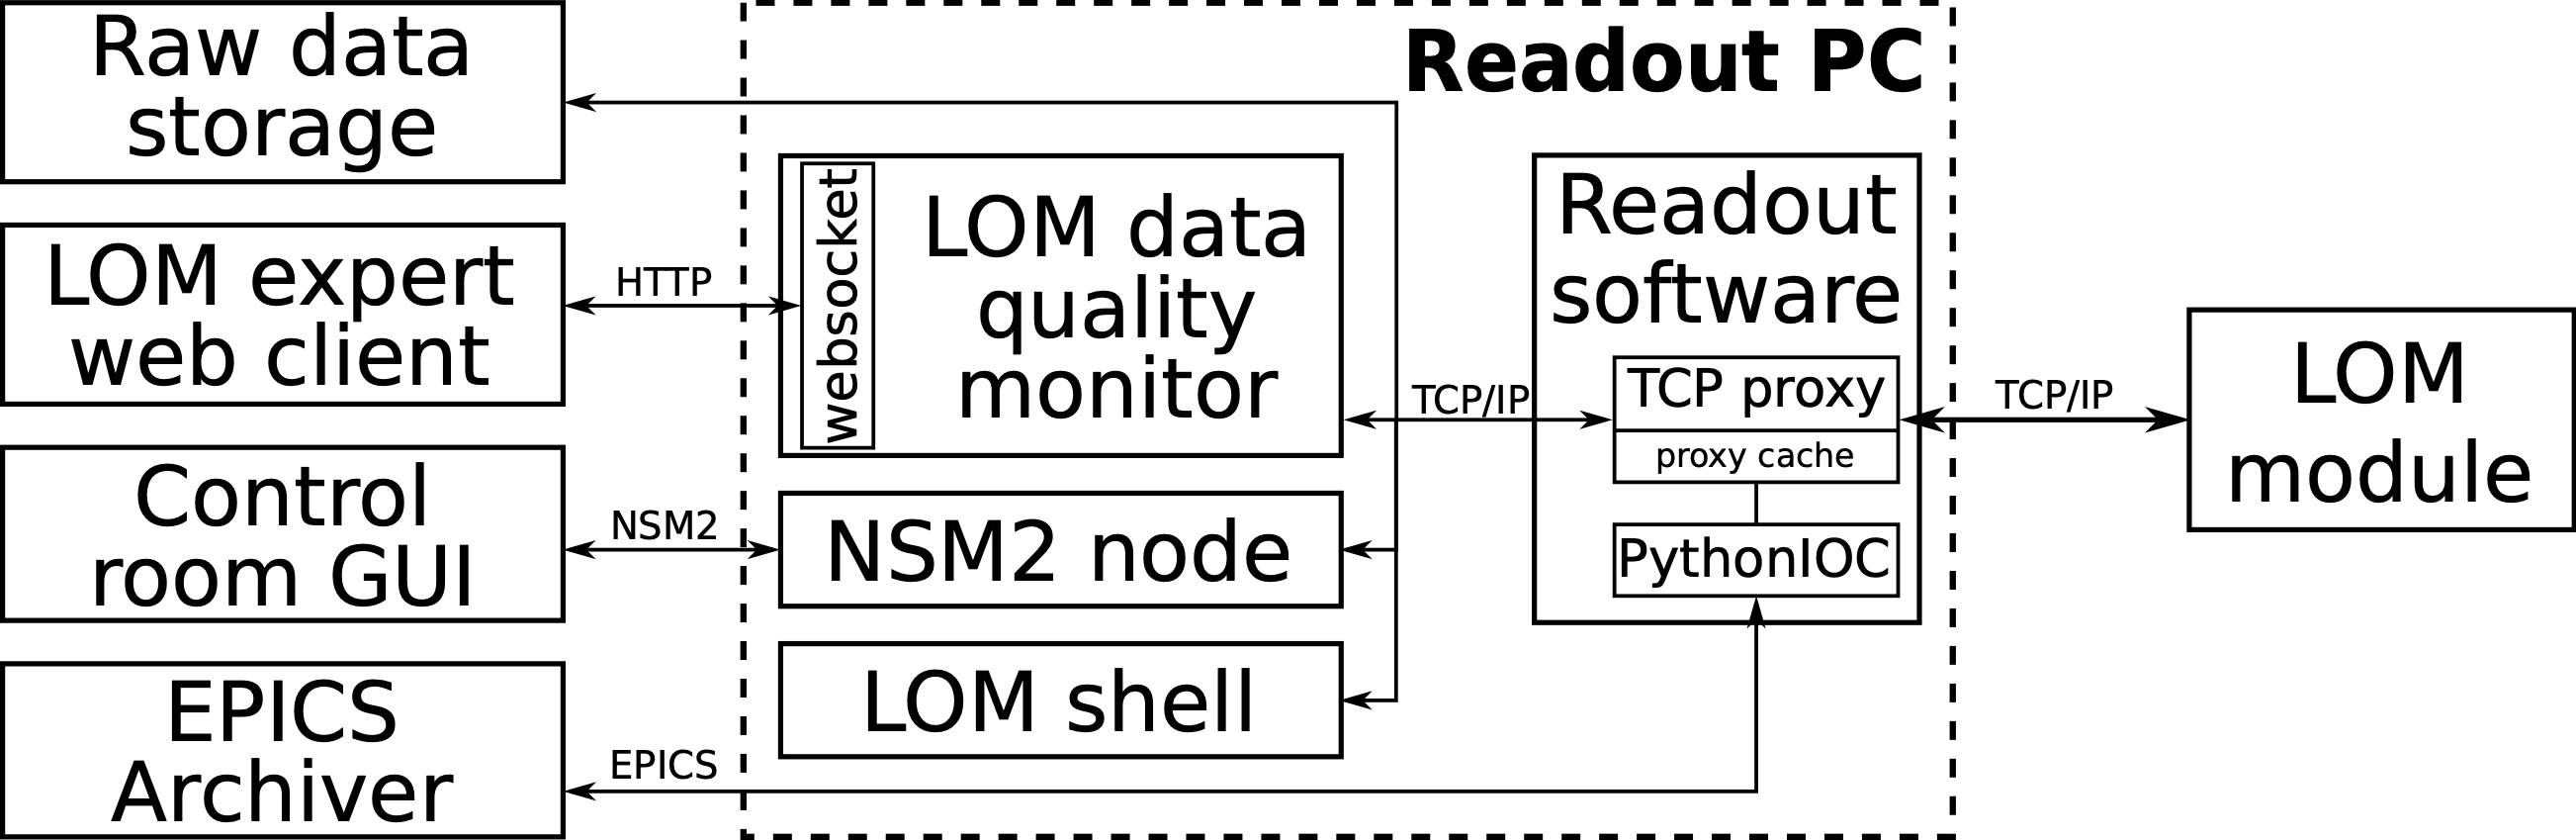
\includegraphics[width=\textwidth]{LOM_software.pdf}
  \caption{Схема архитектуры ПО.}
  \label{fig:galaxy}
\end{figure}

    \subsection{Требования к ПО}
      Для корректного выполнения поставленых к ПО задач, необходимо соблюдать требования выдвигаемые к ПО. Так для ПО онлайн монитора светимости, существуют следующие ребования к его функционированию:
\begin{itemize}
  \item Так как данные с монитора светимости приходят с частотой 1 Гц, то необходимо реализовать обработку данных за время меньшее 1 секунды
  \item Необходимо восстановление накопленных данных при перезагрузке ПО  
  \item Необходимо обнаружение и обработка событий при получении некорректных данных 
  \item Необходимо реализовать поддержку систем медленного контроля NSM2 и EPCIS для хранения данных
  \item ПО должно уметь передавать данные по сети TCP/IP, следовательно необходим протокол взаимодействия с LOM
\end{itemize}


\section{Реализация ПО для онлайн монитора светимости}
%    \subsection{Архитектура ПО}
%      ПО для онлайн монитора светимости работает на выделенном компьютере. Считывающее ПО, запущенное на данном компьютере, непрерывно считывает данные из модуля LOM и позволяет получать значения светимости в локальной сети, а также отправляет полученные значения в системы медленного контроля (Рис. 8). Поскольку поток данных с монитора светимости составляет приблизительно 35 Кб/с, то не накладывается строгих ограничений на производительность считывающего ПО и ПО мониторинга. Также важна скорость разработки ПО и удобство написания многопоточных приложений, работающих с сетью TCP/IP. В связи с этим Python был выбран в качестве основного языка для написания большей части программного обеспечения.\par
  Считывающее ПО представляет собой многопоточный TCP-сервер и работает как прокси для модуля монитора светимости. Поскольку программа ЦПУ монитора светимости является однопоточной, одной из важных функций считывающего ПО является обеспечение обработки поступающих параллельно входящих запросов и предотвращение возможных сбоев прошивки, вызванных несколькими одновременными запросами к монитору светимости. Он также кэширует данные, которые могут запрашиваться клиентскими приложениями, тем самым сокращая количество операций считывания и повышая общую производительность.\par
  Для дальнейшей передачи данных сервер LOM использует библиотеку pythonIOC \cite{PythonIoc}, встроенный сервер доступа к каналам (Channel Access, CA) EPICS, что делает всю информацию о светимости доступной в системе медленного контроля Belle II. Помимо значений мгновенной светимости, он также производит расчет интегральных и максимальных светимостей, значений пьедесталов, обеспечивает сохранность данных, о которых будет описано подробнее в следующей главе.
\begin{figure}[htp]
  \centering
  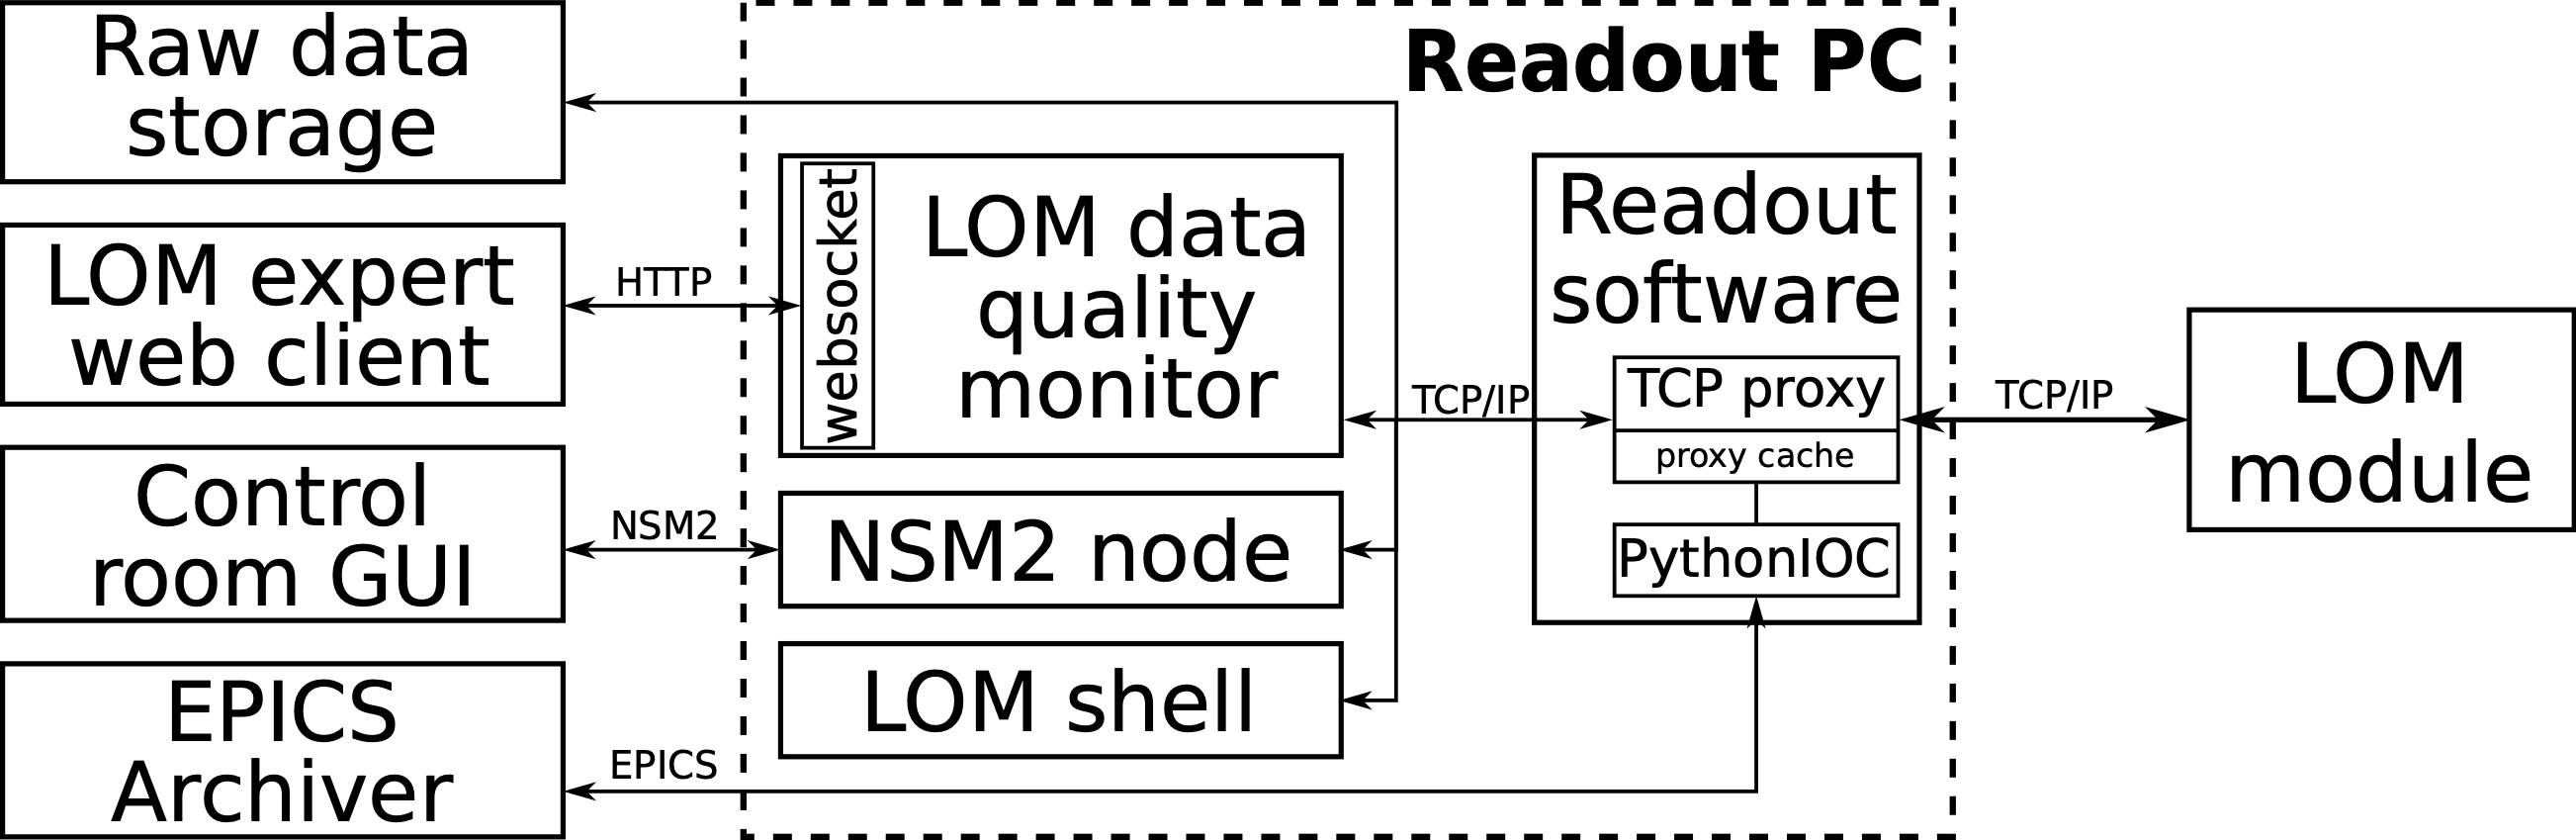
\includegraphics[width=\textwidth]{LOM_software.pdf}
  \caption{Схема архитектуры ПО.}
  \label{fig:galaxy}
\end{figure}

    \subsection{Интегральные и максимальные значения светимостей}
    Здусь будет про светимости

    \subsection{Расчет пьедесталов}
      Так как монитор светимости работает на базе электромагнитного калориметра, то полученные данные можно использовать для получения обратной связи с электромагнитным калориметром в режиме реального времени. Возможность получения обратной связи полезна тем, что можно оперативно обнаружить неисправности в работе электромагнитного калориметра и устранить их. В частности, для мониторирования уровня шумов электроники удобно использовать значения пьедесталов для каждого сектора. В общем случае пьедестал это отклонение уровня сигнала от нулевого положения.\par
  Для каждого из 32 секторов монитор светимости получает аналоговую сумму сигналов с 2 триггерных ячеек. Соответственно, имея форму сигнала, можно определять отклонение от нулевого положения для каждого сектора в режиме реального времени. Форма сигнала представляет собой массив из 2048 значений на один сектор. Расчет происходит следующим образом:
\begin{enumerate}
  \item Считываем формы сигналов с монитора светимости
  \item Находим максимальное значение в массиве
  \item Проверяем, превышает ли максимальное значение установленное пороговое (устанавливаем, было ли событие в данном секторе)
  \item Если максимальное значение превышает пороговое, то необходимо удалить 50 значений слева от максимума и 150 справа (Рис. 9). Иначе, переходим к следующему пункту
  \item Считаем среднее арифметическое по оставшимся значениям
\end{enumerate}
Данный алгоритм повторяем для каждого сектора. Все полученные значения пьедесталов сохраняются в систему медленного контроля EPICS.
\begin{figure}[htp]
  \centering
  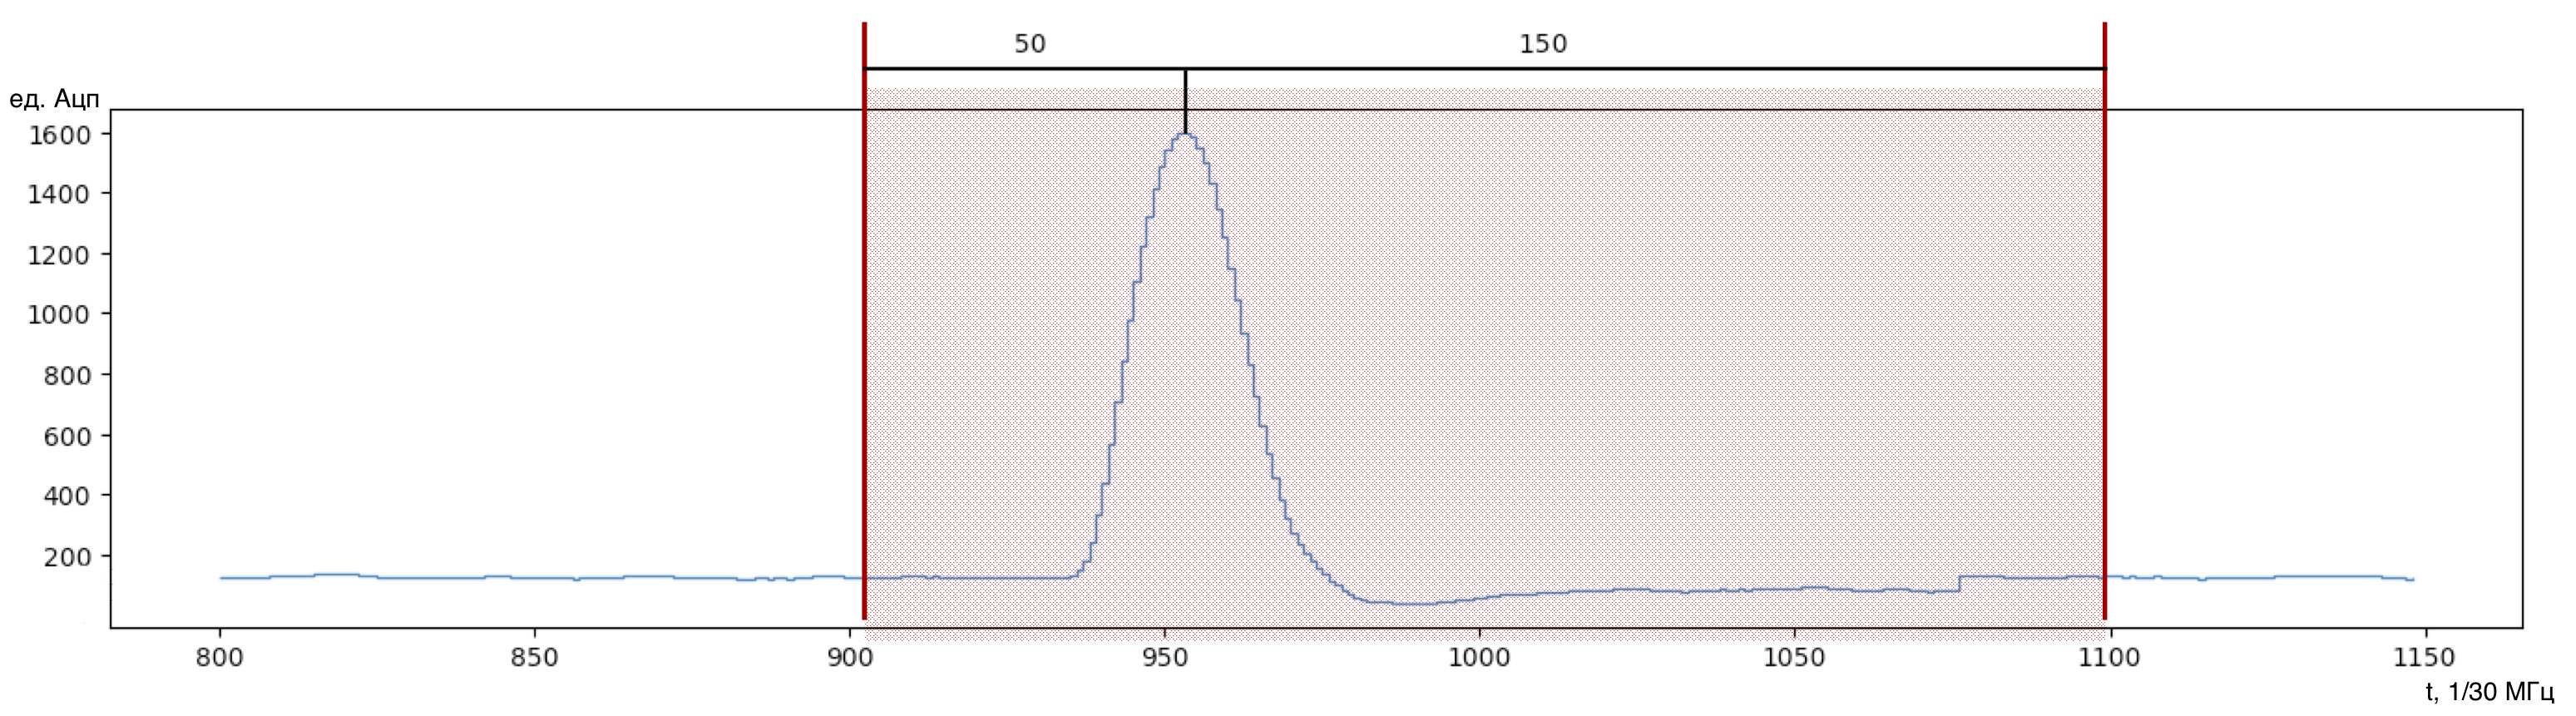
\includegraphics[width=\textwidth]{Pedestal}
  \caption{Схема расчета значений пьедесталов.}
  \label{fig:galaxy}
\end{figure}

    \subsection{Графический интерфейс}
    Здесь будет про графический интерфейс

    \subsection{Автоматизация энергетической калибровки LOM}
      Формы сигналов, которые получает монитор светимости имеют размерность в единицах АЦП на канал. Необходимо получать значения в энергетических единицах. Следовательно, стоит задача определения цены деления АЦП для каждого канала. Для этой цели была разработана процедура энергетической калибровки онлайн монитора светимости. Процедура основывается на посылке тестового сигнала и сравнения амплитуд с монитора светимости и уже откалиброванной системой DAQ. Калибровочные коэффициенты рассчитываются следующим образом:
\begin{equation}
  \eta = \frac{A_{DAQ}}{A_{LOM}}
\end{equation}
 где $A_{DAQ}$ и $A_{LOM}$ амплитуды с системы сбора данных DAQ и монитора светимости соответственно.\par
  Подробная схема данной процедуры представлена на рисунке 11 и заключается в следующем:
\begin{enumerate}
  \item На электромагнитный калориметр при помощи генератора импульсов подается тестовый сигнал
  \item Далее сигнал проходит все системы до монитора светимости как реальный сигнал
  \item На выходе с монитора светимости получаем амплитудные значения в каналах АЦП
  \item Далее вычисляются калибровочные коэффициенты по формуле (2)
\end{enumerate}\par
\begin{figure}[htp]
  \centering
  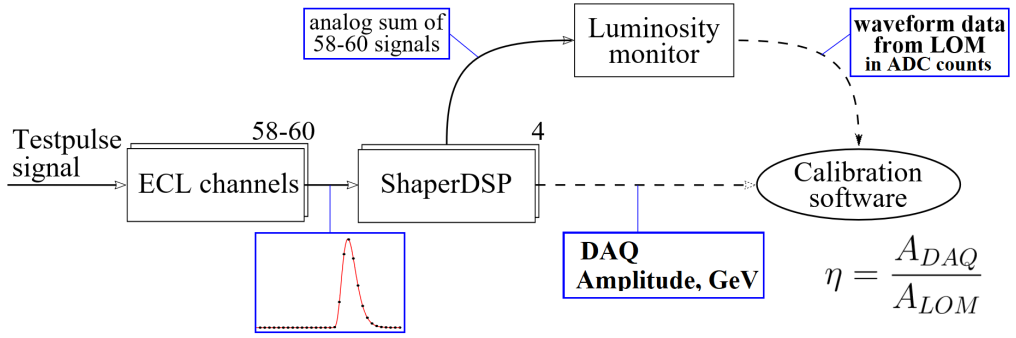
\includegraphics[width=\textwidth]{calibration.png}
  \caption{Процесс энергетической калибровки монитора светимости.}
  \label{fig:galaxy}
\end{figure}
  Так как в процессе энергетической калибровки необходимо параллельно читать данные с монитора светимости и амплитудные значения с системы сбора данных DAQ, то нужно иметь возможность управлять чтением данных с монитора светимости. Требуется останавливать и продолжать чтение данных в любой момент времени. Для реализации данной возможности был расширен протокол монитора светимости. Были добавлены команды, которые позволяют остановить чтение данных с монитора светимости, возобновить чтение данных и посмотреть текущий статус монитора светимости.\par
  Также для автоматизации контроля актуальной версии калибровочных коэффициентов, было реализовано хранение калибровочных коэффициентов в базе данных DAQ. При запуске ПО находит последнюю версию калибровочных коэффициентов и использует их в дальнейшем.\par
  В торцах электромагнитного калориметра находится 2112 кристаллов, однако, монитор светимости в конечном итоге получает суммированную информацию с этих каналов, сгруппированную по 32 секторам. Таким образом форма сигнала для каждого сектора -- это сумма форм сигналов от, в среднем, 2112/32 = 66 каналов. Однако, все кристаллы обладают немного разными физическими характеристиками, в частности, разным световыходом, требуется суммировать сигналы с неким весом. Этот вес называется коэффициентом аттенюации. Проанализировав изменения аттенюаторных и калибровочных коэффициентов, было замечено, что они коррелируют друг с другом. Поэтому, для более детального анализа, было проведен анализ изменения аттенюаторных коэффициентов и калибровочных за одинаковые промежутки времени. Результат сравнения представлен на рисунке 12. Таким образом, можно проверять, если изменились аттенюаторные коэффициенты, то на соответствующую величину изменять и калибровочные коэффициенты. Видно, что для некоторых секторов, к примеру секторов 1 и 28, корреляция не наблюдается, поэтому процедура автоподстройки коэффициентов является только вспомогательной операцией по отношению к калибровке. Тем не менее, эта процедура позволяет точнее исследовать вклад различных факторов, влияющих на цену деления АЦП.\par
  Также в случае возникновения проблем с соединением или считыванием значений из базы данных в компьютере, на котором запущено ПО, имеется офлайн версия калибровочных коэффициентов. Такой подход позволяет функционировать ПО независимо от соединения с БД.
\begin{figure}[htp]
  \centering
  \includegraphics[width=\textwidth]{coefs_new.pdf}
  \caption{Изменение калибровочных и аттенюаторных коэффициентов за равный промежуток времени.}
  \label{fig:galaxy}
\end{figure}


\section*{Заключение}
\addcontentsline{toc}{section}{Заключение}
    В рамках данной работы было улучшено ПО для онлайн монитора светимости:
    \begin{itemize}
        \item Изменена архитектура ПО, что позволило увеличить стабильность работы системы. При помощи библиотеки pythonIOC реализована параллельная передача данных в системы медленного контроля NSM2 и EPICS.
        \item Добавлен расчет интегральной и максимальной светимостей за характерные промежутки времени.
        \item Добавлен расчет значений пьедесталов для каждого сектора, значения высчитываются в режиме реального времени.
        \item Создана база данных на основе sqlite для сохранения текущих значений светимостей, также записываются значение светимостей за предыдущие заходы.
        \item Расширен протокол управления монитором светимости. Реализованы команды pause и continue.
        \item Добавлено считывание значений калибровочных коэффициентов из базы данных при запуске
    \end{itemize}
    
    Также был улучшен графический интерфейс для монитора светимости, который позволяет проводить удаленную настройку параметров, а также визуализирует данные с монитора светимости
    \begin{itemize} 
        \item Добавлено отображение значений пьедесталов для каждого сектора.
        \item Добавлено считывание порогового значения амплитуд для каждого сектора.
        \item Также были исправлены незначительные ошибки и улучшен интерфейс.
    \end{itemize}
    
    Также была написана программа для отображения основных параметров с монитора светимости, которую планируется интегрировать с веб-сервером?
\section*{Список литературы}
\addcontentsline{toc}{section}{Список литературы}

\end{document}
